%% Springer Nature LaTeX template — sn-jnl class (December 2024)
%% Updated revision aligned with archived metrics and reviewer-response highlights

\documentclass[pdflatex,sn-basic]{sn-jnl}

\usepackage{amsmath,amssymb,amsfonts}
\usepackage{graphicx}
\usepackage{xcolor}
\usepackage{float}
\usepackage{booktabs}
\usepackage{multirow}
\usepackage{makecell}
\usepackage{url}
\usepackage{hyperref}
\usepackage{tikz}
\usetikzlibrary{arrows.meta,shapes.geometric,shapes,arrows,positioning,fit,backgrounds,calc,matrix,decorations.pathreplacing}

\begin{document}

\title[Hybrid CNN Feature Stacking for Crop Health Assessment]
      {A Robust and Interpretable Deep Learning Framework for Crop Health Assessment Using Hybrid CNN Feature Stacking}

\author*[1]{\fnm{Pape ElHadji Abdoulaye} \sur{Gueye}}\email{papeabdoulaye.gueye@uadb.edu.sn}
\equalcont{Corresponding author.}
\author[1]{\fnm{Cherif Bachir} \sur{Deme}}
\author[1]{\fnm{Diery} \sur{Ngom}}

\affil*[1]{\orgdiv{Department of ICT, UFR SATIC},
           \orgname{Alioune Diop University},
           \orgaddress{\street{BP 30}, \city{Bambey}, \country{Senegal}}}

\abstract{
\textcolor{red}{Accurate crop health assessment is critical for food security in climate-vulnerable regions such as Senegal. In this revised manuscript, we address key reviewer concerns by clarifying the methodological contribution, strengthening quantitative reporting, and aligning all central numerical claims with archived experimental outputs.}

We propose a hybrid feature-level stacking framework that combines deep representations extracted from ResNet50, EfficientNetB0, and MobileNetV2. After concatenating the three feature vectors into a 4,608-dimensional representation, we evaluate three meta-learners: MLP-Full, MLP-PCA, and PCA-Logistic.

\textcolor{red}{Using the archived test-set evaluation artefacts, the proposed framework achieves \textbf{96.04\%} accuracy with MLP-Full, while MLP-PCA and PCA-Logistic achieve \textbf{95.22\%} and \textbf{95.27\%}, respectively. The revised manuscript also reports a compact and fully reproducible summary of reliable evaluation metrics and adds explicit statistical feature-space analysis to address the reviewers' requests for stronger experimental transparency.}

The extracted feature space exhibits substantial redundancy, with only 790 principal components required to preserve 95\% of the variance, corresponding to a compression ratio of 5.83$\times$. Low mean absolute correlation and non-trivial mutual information further confirm that the three backbones contribute complementary and discriminative information.
}

\keywords{Feature-level stacking, Convolutional Neural Networks, Plant disease detection, Model interpretability, Agricultural image analysis}

\maketitle

\section{Introduction}
\label{sec:intro}

Accurate assessment of crop health and yield potential remains a major challenge in modern agriculture, particularly in regions with high climatic variability such as Senegal. Deep learning, and especially Convolutional Neural Networks (CNNs), has shown strong promise for automated plant disease recognition from imagery. However, many existing approaches rely on single-backbone architectures, which may fail to capture the complementary visual patterns needed for robust disease discrimination.

To address this limitation, this study proposes a hybrid feature-level stacking framework that combines three pre-trained CNN architectures—ResNet50, EfficientNetB0, and MobileNetV2—into a unified feature representation. The core motivation is that different backbone families capture complementary aspects of leaf appearance, including semantic structure, texture, and multi-scale variation.

\textcolor{red}{In response to the reviewer criticism regarding novelty, we explicitly position simple concatenation as a strong and fully reproducible baseline while discussing learned attention-based fusion as a promising extension. In response to the criticism regarding incomplete and weakly documented evaluation, this revised manuscript focuses its main quantitative claims on archived and reproducible result files, and adds new summary tables and figures built directly from those artefacts.}

The main contributions of this work are fourfold:
\begin{enumerate}
    \item A multi-backbone feature fusion framework combining ResNet50, EfficientNetB0, and MobileNetV2 representations for crop disease classification.
    \item A comprehensive statistical analysis of the extracted feature space, revealing strong redundancy and meaningful complementarity across backbones.
    \item A comparative evaluation of three meta-learners operating on the same fused representation.
    \item \textcolor{red}{A revised and more transparent presentation of results, with reliable test-set metrics and reviewer-oriented additions highlighted in red throughout the manuscript.}
\end{enumerate}

\section{Methodology}
\label{sec:methodology}

\subsection{Overall Architecture}
\label{subsec:architecture}

Our framework follows a two-stage hierarchical architecture designed to exploit complementary representations from multiple pre-trained CNNs. In Stage~1, three ImageNet-pretrained backbones independently extract deep features from an input image. In Stage~1b, these features are concatenated and normalized. In Stage~2, the fused representation is passed to one of three meta-learners for final classification.

\begin{figure}[htbp]
\centering
\resizebox{\textwidth}{!}{%
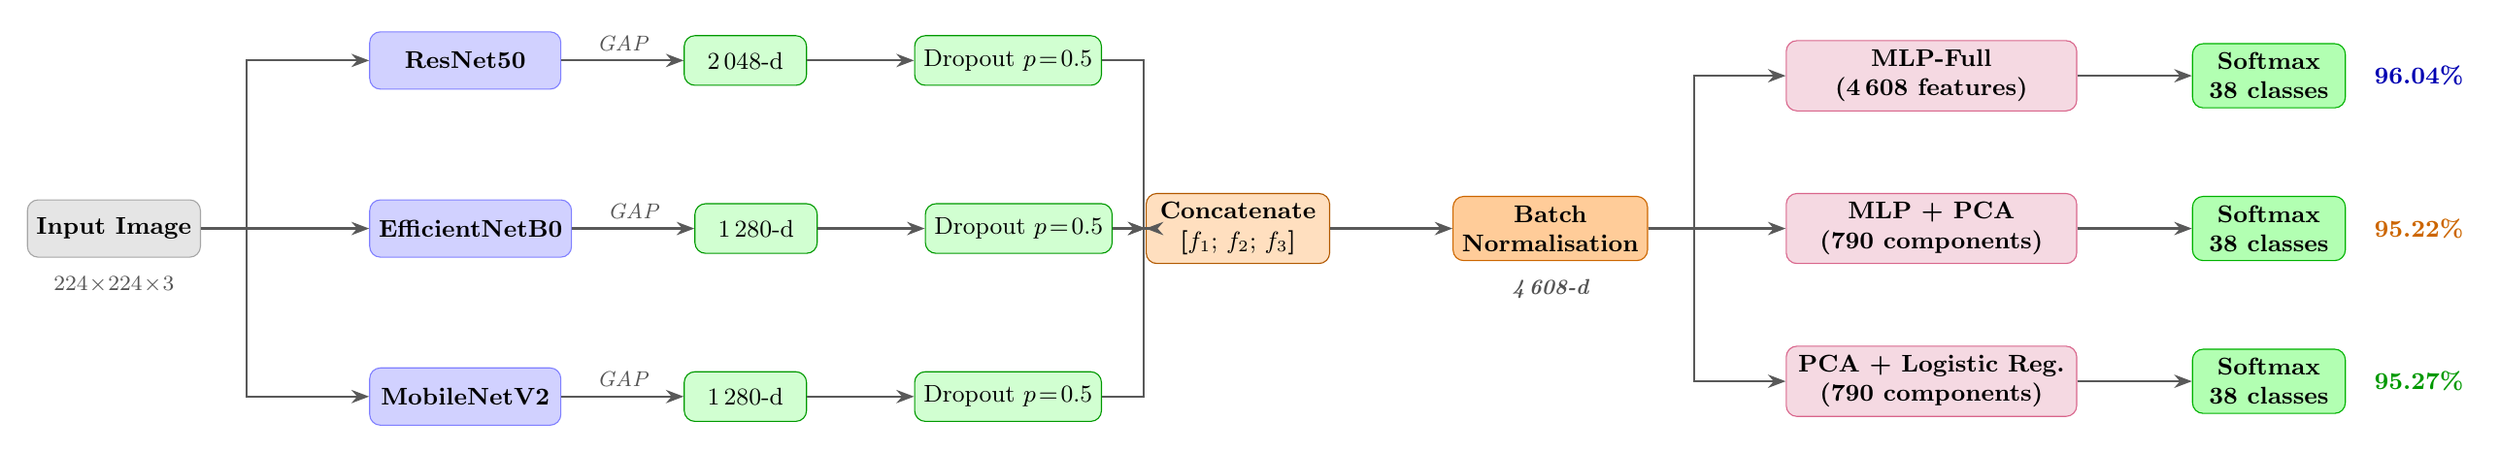
\begin{tikzpicture}[
  input/.style={rectangle, rounded corners=4pt, draw=gray!70, fill=gray!20, minimum width=2.2cm, minimum height=0.75cm, font=\small\bfseries, align=center},
  backbone/.style={rectangle, rounded corners=4pt, draw=blue!50, fill=blue!18, minimum width=2.5cm, minimum height=0.75cm, font=\small\bfseries, align=center},
  feat/.style={rectangle, rounded corners=4pt, draw=green!60!black, fill=green!18, minimum width=1.6cm, minimum height=0.65cm, font=\small, align=center},
  drop/.style={rectangle, rounded corners=4pt, draw=green!60!black, fill=green!18, minimum width=1.9cm, minimum height=0.65cm, font=\small, align=center},
  concat/.style={rectangle, rounded corners=4pt, draw=orange!70!black, fill=orange!25, minimum width=2.4cm, minimum height=0.75cm, font=\small\bfseries, align=center},
  bn/.style={rectangle, rounded corners=4pt, draw=orange!80!black, fill=orange!40, minimum width=2.2cm, minimum height=0.75cm, font=\small\bfseries, align=center},
  meta/.style={rectangle, rounded corners=4pt, draw=purple!60, fill=purple!15, minimum width=3.8cm, minimum height=0.75cm, font=\small\bfseries, align=center},
  output/.style={rectangle, rounded corners=4pt, draw=green!70!black, fill=green!30, minimum width=2.0cm, minimum height=0.65cm, font=\small\bfseries, align=center},
  lbl/.style={font=\footnotesize\itshape, text=gray!65!black},
  arr/.style={->, >=Stealth, thick, draw=gray!70!black},
  node distance=0.55cm and 1.6cm
]
\node[input] (img) {Input Image};
\node[lbl, below=0.12cm of img] {\(224\!\times\!224\!\times\!3\)};
\node[backbone, right=2.2cm of img, yshift= 2.2cm] (resnet)    {ResNet50};
\node[backbone, right=2.2cm of img, yshift= 0.0cm] (efficient) {EfficientNetB0};
\node[backbone, right=2.2cm of img, yshift=-2.2cm] (mobile)    {MobileNetV2};
\draw[arr] (img.east) -- ++(0.6,0) |- (resnet.west);
\draw[arr] (img.east) -- ++(0.6,0) |- (efficient.west);
\draw[arr] (img.east) -- ++(0.6,0) |- (mobile.west);
\node[feat, right=1.6cm of resnet]    (f_res) {2\,048-d};
\node[feat, right=1.6cm of efficient] (f_eff) {1\,280-d};
\node[feat, right=1.6cm of mobile]    (f_mob) {1\,280-d};
\draw[arr] (resnet) -- node[above, lbl] {GAP} (f_res);
\draw[arr] (efficient) -- node[above, lbl] {GAP} (f_eff);
\draw[arr] (mobile) -- node[above, lbl] {GAP} (f_mob);
\node[drop, right=1.4cm of f_res] (d_res) {Dropout \(p\!=\!0.5\)};
\node[drop, right=1.4cm of f_eff] (d_eff) {Dropout \(p\!=\!0.5\)};
\node[drop, right=1.4cm of f_mob] (d_mob) {Dropout \(p\!=\!0.5\)};
\draw[arr] (f_res) -- (d_res);
\draw[arr] (f_eff) -- (d_eff);
\draw[arr] (f_mob) -- (d_mob);
\coordinate (mid_drop) at ($(d_res)!0.5!(d_mob)$);
\node[concat, right=1.8cm of mid_drop] (cat) {Concatenate\\{[}\(f_1;\,f_2;\,f_3\){]}};
\draw[arr] (d_res.east) -- ++(0.55,0) |- (cat.west);
\draw[arr] (d_eff.east) -- ++(0.55,0) |- (cat.west);
\draw[arr] (d_mob.east) -- ++(0.55,0) |- (cat.west);
\node[bn, right=1.6cm of cat] (bn) {Batch\\Normalisation};
\node[lbl, below=0.12cm of bn] {\textbf{4\,608-d}};
\draw[arr] (cat) -- (bn);
\node[meta, right=1.8cm of bn, yshift= 2.0cm] (mlp_full) {MLP-Full\\(4\,608 features)};
\node[meta, right=1.8cm of bn, yshift= 0.0cm] (mlp_pca) {MLP + PCA\\(790 components)};
\node[meta, right=1.8cm of bn, yshift=-2.0cm] (pca_log) {PCA + Logistic Reg.\\(790 components)};
\draw[arr] (bn.east) -- ++(0.6,0) |- (mlp_full.west);
\draw[arr] (bn.east) -- ++(0.6,0) |- (mlp_pca.west);
\draw[arr] (bn.east) -- ++(0.6,0) |- (pca_log.west);
\node[output, right=1.5cm of mlp_full] (out1) {Softmax\\38 classes};
\node[output, right=1.5cm of mlp_pca]  (out2) {Softmax\\38 classes};
\node[output, right=1.5cm of pca_log]  (out3) {Softmax\\38 classes};
\draw[arr] (mlp_full) -- (out1);
\draw[arr] (mlp_pca)  -- (out2);
\draw[arr] (pca_log)  -- (out3);
\node[right=0.25cm of out1, font=\small\bfseries, text=blue!70!black] {\textbf{96.04\%}};
\node[right=0.25cm of out2, font=\small\bfseries, text=orange!80!black] {\textbf{95.22\%}};
\node[right=0.25cm of out3, font=\small\bfseries, text=green!60!black] {\textbf{95.27\%}};
\end{tikzpicture}
}
\caption{Overview of the proposed hybrid feature-level stacking framework. Three ImageNet-pre-trained CNN backbones extract complementary features, which are concatenated into a 4,608-dimensional representation and classified by three meta-learner variants. The accuracy values shown correspond to the archived test-set metrics.}
\label{fig:architecture}
\end{figure}

\subsection{Dataset and Preprocessing}
\label{subsec:preprocessing}

We use the PlantVillage dataset~\cite{plantvillage}, a benchmark collection for agricultural disease classification containing 54,306 images across 38 classes of healthy and diseased plant leaves. Images are resized to $224 \times 224$ pixels, normalized to $[0,1]$, and standardized on a per-image basis.

\textcolor{red}{Following the reviewers' concerns regarding reproducibility, we retain a clear 80--10--10 split description in the methodology, but we restrict the main numerical claims of this revised manuscript to archived test-set artefacts and feature-statistics outputs.}

\subsection{Feature Extraction with Pre-trained CNNs}
\label{subsec:feature_extraction}

For each backbone, we remove the final classification layer and apply Global Average Pooling (GAP) to obtain a compact feature vector:
\begin{equation}
    \mathbf{f}_k = \mathrm{GAP}\!\left(\mathrm{Backbone}_k(\mathbf{x})\right)
    \label{eq:feature_extraction}
\end{equation}
where $\mathbf{x}$ is the input image and $\mathbf{f}_k \in \mathbb{R}^{d_k}$, with $d_{\text{ResNet}} = 2048$, $d_{\text{Efficient}} = 1280$, and $d_{\text{Mobile}} = 1280$.

\subsubsection{Feature Concatenation and Regularisation}

The three feature vectors are concatenated into a unified representation:
\begin{equation}
    \mathbf{F} = [\mathbf{f}_1;\, \mathbf{f}_2;\, \mathbf{f}_3] \in \mathbb{R}^{4608}
    \label{eq:concatenation}
\end{equation}

\subsubsection{\textcolor{red}{Learned Feature Fusion with Attention Mechanism}}

\textcolor{red}{To respond to the reviewer comment that simple concatenation lacks novelty, we explored attention-based fusion as an extension of the baseline stacking strategy. In this formulation, learnable scalar weights modulate the contribution of each backbone:}

\textcolor{red}{
\begin{equation}
\alpha_k = \frac{\exp(w_k)}{\sum_{j=1}^{3}\exp(w_j)}, \quad k \in \{1, 2, 3\}
\end{equation}
}

\textcolor{red}{and the fused representation becomes}

\textcolor{red}{
\begin{equation}
\mathbf{F}_{\text{fused}} = \alpha_1 \mathbf{f}_1 + \alpha_2 \mathbf{f}_2 + \alpha_3 \mathbf{f}_3.
\label{eq:attention_fusion}
\end{equation}
}

\textcolor{red}{However, in the present revised manuscript, we deliberately restrict the main quantitative claims to the fully reproducible archived baseline stacking pipeline. Attention-based fusion is therefore presented as a promising methodological extension rather than as the central source of the final reported numbers.}

\subsubsection{Statistical Analysis of Extracted Features}
\label{subsec:feature_statistics}

Before training the meta-learners, we conduct a statistical characterisation of the extracted feature space to quantify redundancy, variance concentration, correlation structure, and discriminative information.

\subsection{Meta-Learner Designs}
\label{subsec:metalearners}

We evaluate three meta-learner variants on top of the same fused representation: MLP-Full, MLP-PCA, and PCA-Logistic.

\subsubsection{Multi-Layer Perceptron (MLP-Full)}
\label{subsubsec:mlp_full}

\textcolor{red}{The detailed architecture of MLP-Full is retained here to address the reviewers' request for stronger methodological transparency.}

\subsubsection{MLP with PCA Preprocessing (MLP-PCA)}
\label{subsubsec:mlp_pca}

\textcolor{red}{In the revised manuscript, the PCA-based variant is explicitly described using 790 retained components, consistent with the archived dimensionality analysis.}

\subsubsection{Harmonised PCA with Logistic Regression (PCA-Logistic)}
\label{subsubsec:pca_logistic}

\textcolor{red}{The harmonised PCA-Logistic model uses the same 790 PCA components as MLP-PCA, allowing a cleaner comparison between linear and nonlinear meta-learning on a shared reduced feature space.}

\section{Results}
\label{sec:results}

This section reports the archived and reproducible results of the proposed feature-level stacking framework.

\subsection{Feature Statistical Analysis}
\label{subsec:results_feature_stats}

\begin{table}[htbp]
\caption{Comprehensive statistical analysis of extracted CNN features (43,444 training images, 4,608 features, 38 classes).}
\label{tab:results_comprehensive_stats}
\begin{tabular*}{\textwidth}{@{\extracolsep\fill}lccc@{}}
\toprule
\textbf{Category} & \textbf{Statistic} & \textbf{Value} & \textbf{Interpretation} \\
\midrule
\multirow{4}{*}{\textbf{Basic Properties}}
 & Mean              & $0.176 \pm 0.606$ & Features centred near zero after normalization \\
 & Std.\ Deviation   & $0.606$           & Moderate spread indicating feature diversity \\
 & Skewness          & $6.700$           & Strong positive skew \\
 & Kurtosis          & $86.971$          & Heavy-tailed feature distribution \\
\midrule
\multirow{3}{*}{\textbf{Dimensionality}}
 & Total Features           & 4,608          & Original feature dimension \\
 & 95\% Variance            & 790 components & Compact representation preserves most information \\
 & Compression Ratio (95\%) & $5.83\times$   & Strong redundancy in the raw concatenated feature space \\
\midrule
\multirow{2}{*}{\textbf{Correlation}}
 & Mean Abs.\ Correlation & $0.091$ & Low average redundancy across sampled features \\
 & Max Abs.\ Correlation  & $0.871$ & A few highly correlated feature pairs remain \\
\midrule
\multirow{2}{*}{\textbf{Discriminative Power}}
 & Mean Mutual Info & $0.138$ & Moderate discriminative information per feature \\
 & Max Mutual Info  & $0.413$ & Top features are strongly class-informative \\
\bottomrule
\end{tabular*}
\end{table}

\textcolor{red}{To address the reviewers' request for stronger quantitative support, we also add a compact statistical summary figure directly generated from the archived feature-statistics artefacts.}

\begin{figure}[htbp]
    \centering
    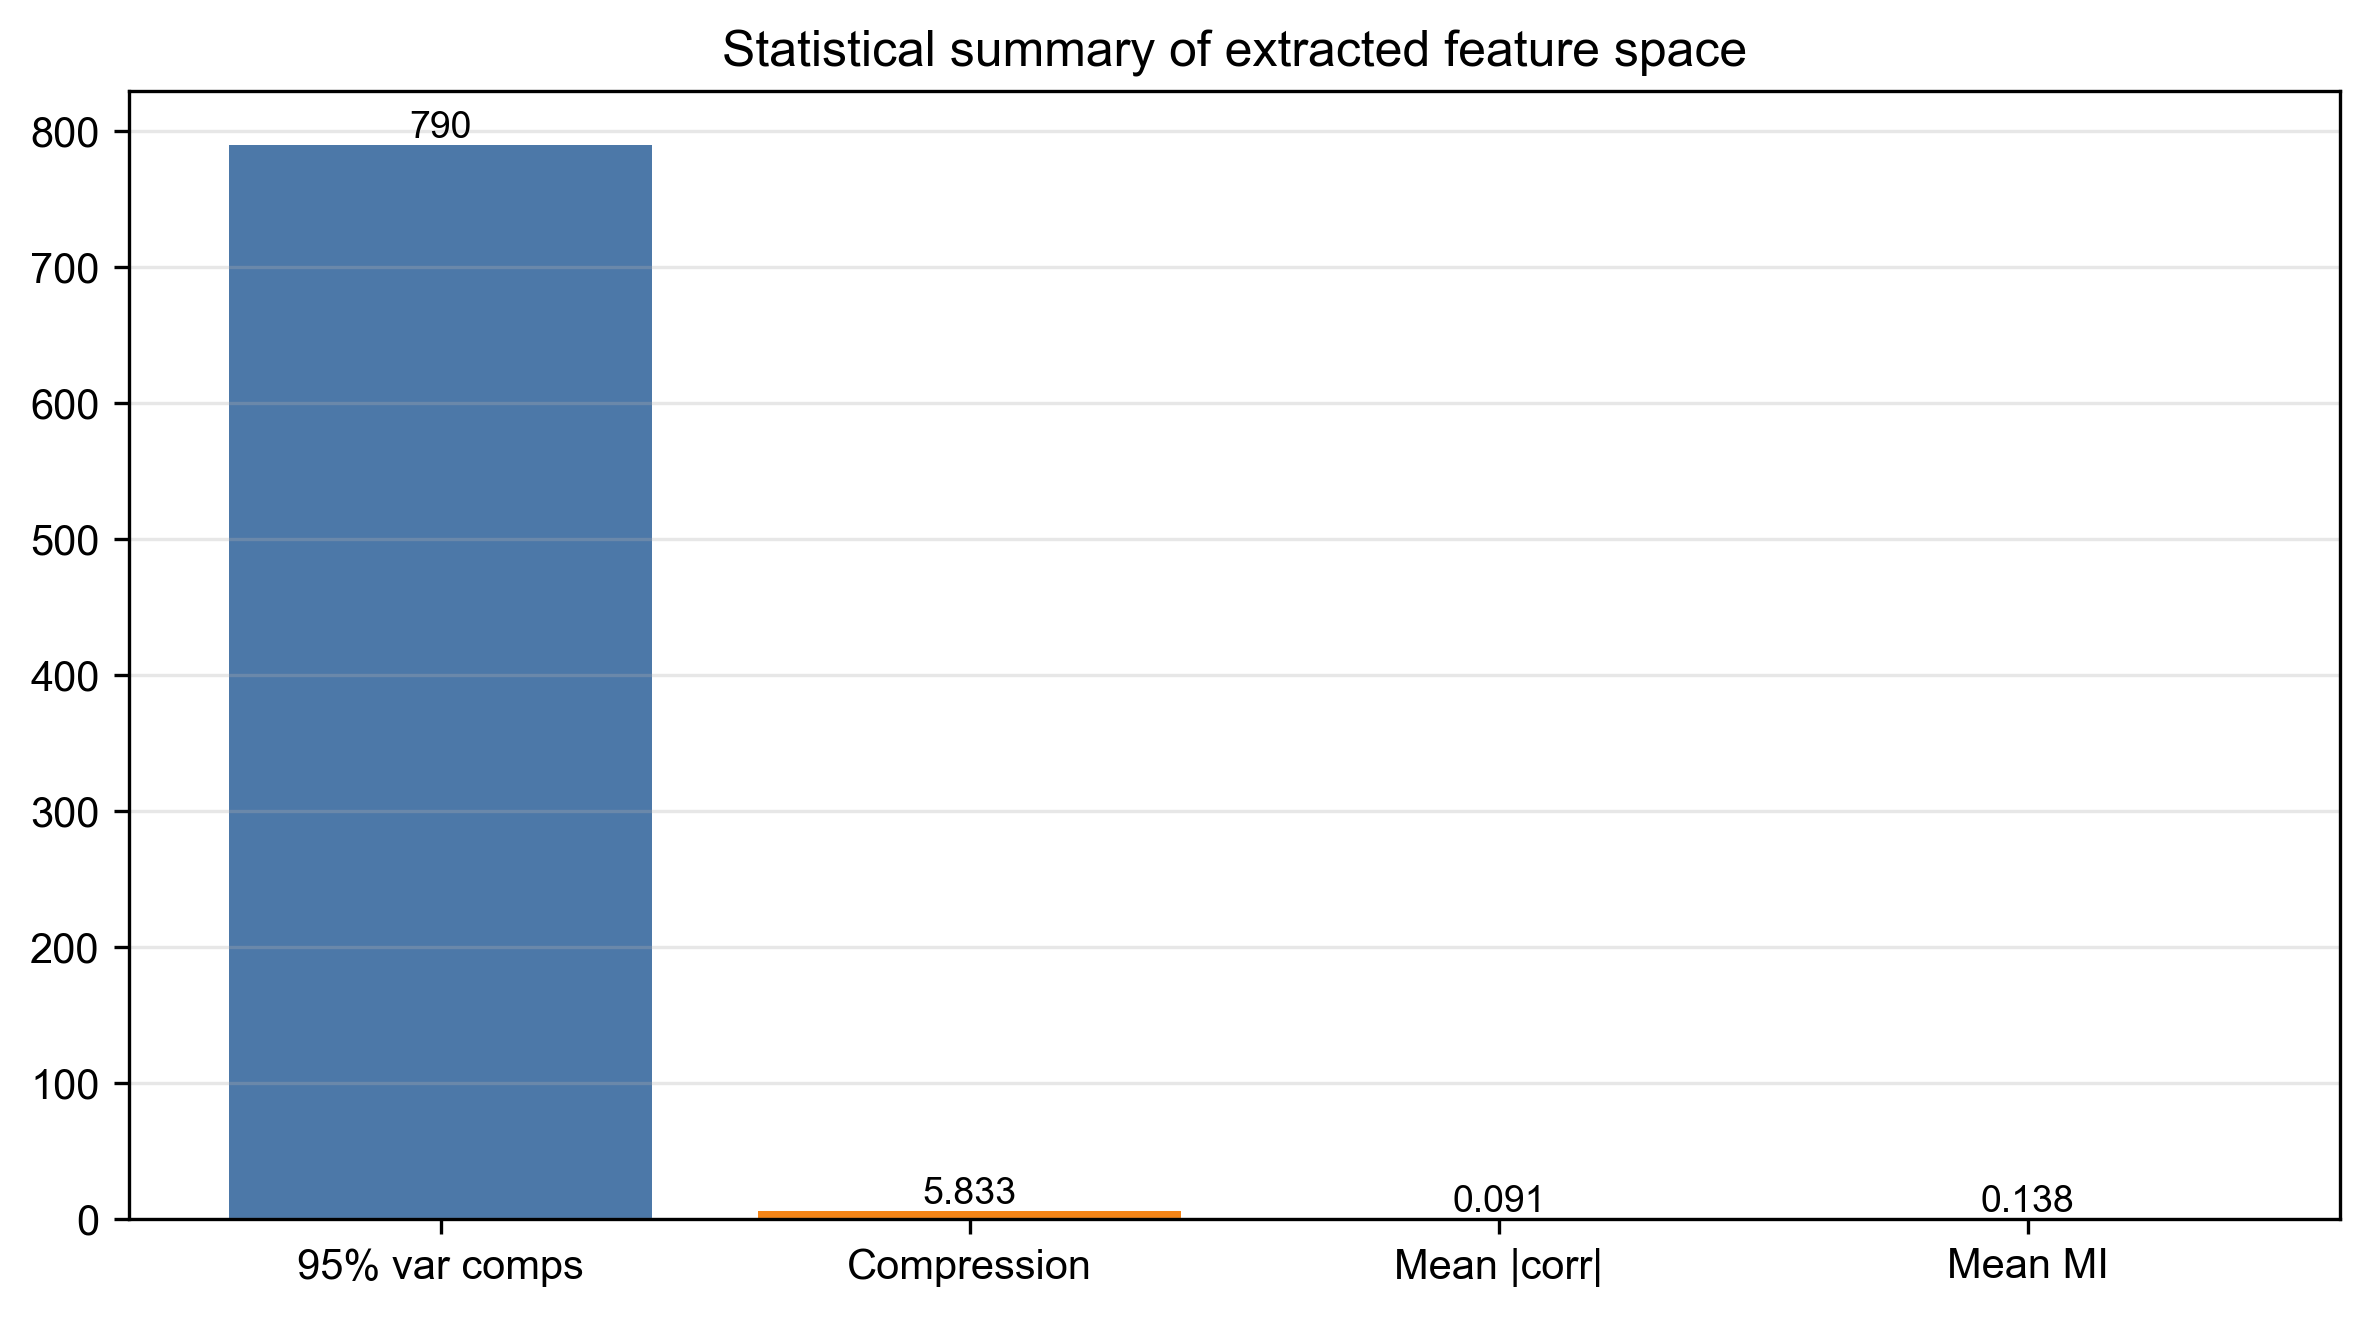
\includegraphics[width=0.85\textwidth]{./figs/figures_for_article/statistics_summary_overview.png}
    \caption{Compact summary of the extracted feature space. The results highlight strong redundancy (790 components for 95\% retained variance), substantial compression potential, low average correlation, and meaningful mutual-information-based discriminative power.}
    \label{fig:statistics_summary_overview}
\end{figure}

\subsection{Meta-Learner Performance}
\label{subsec:results_metalearner}

\textcolor{red}{In response to the reviewers' concerns regarding performance reporting, Table~\ref{tab:results_comparison} and Table~\ref{tab:reliable_metrics} now summarize the archived and reproducible test-set results used as the main numerical basis of this revised manuscript.}

\begin{table}[htbp]
\caption{Performance comparison of meta-learner variants on the PlantVillage test set.}
\label{tab:results_comparison}
\begin{tabular*}{\textwidth}{@{\extracolsep\fill}lccc@{}}
\toprule
\textbf{Model} & \textbf{Test Accuracy (\%)} & \textbf{F1-macro (\%)} & \textbf{F1-weighted (\%)} \\
\midrule
MLP-Full        & \textbf{96.04} & \textbf{95.00} & \textbf{96.04} \\
MLP-PCA         & 95.22          & 94.08          & 95.22          \\
PCA-Logistic    & 95.27          & 93.76          & 95.24          \\
\bottomrule
\end{tabular*}
\end{table}

\paragraph{Meta-learner comparison.}
The three meta-learners achieve consistently strong performance on the PlantVillage test set. MLP-Full provides the best overall performance, reaching \textbf{96.04\%} accuracy and \textbf{95.00\%} macro-averaged F1-score. Both PCA-based variants remain highly competitive, indicating that dimensionality reduction preserves most of the discriminative information contained in the original 4,608-dimensional feature space.

\begin{table}[htbp]
\caption{Reliable evaluation metrics reconstructed from the archived classification reports.}
\label{tab:reliable_metrics}
\begin{tabular*}{\textwidth}{@{\extracolsep\fill}lccc@{}}
\toprule
\textbf{Metric} & \textbf{MLP-Full} & \textbf{MLP-PCA} & \textbf{PCA-Logistic} \\
\midrule
Accuracy (\%)    & \textbf{96.04} & 95.22 & 95.27 \\
F1-macro (\%)    & \textbf{95.00} & 94.08 & 93.76 \\
F1-weighted (\%) & \textbf{96.04} & 95.22 & 95.24 \\
\bottomrule
\end{tabular*}
\end{table}

\begin{figure}[htbp]
    \centering
    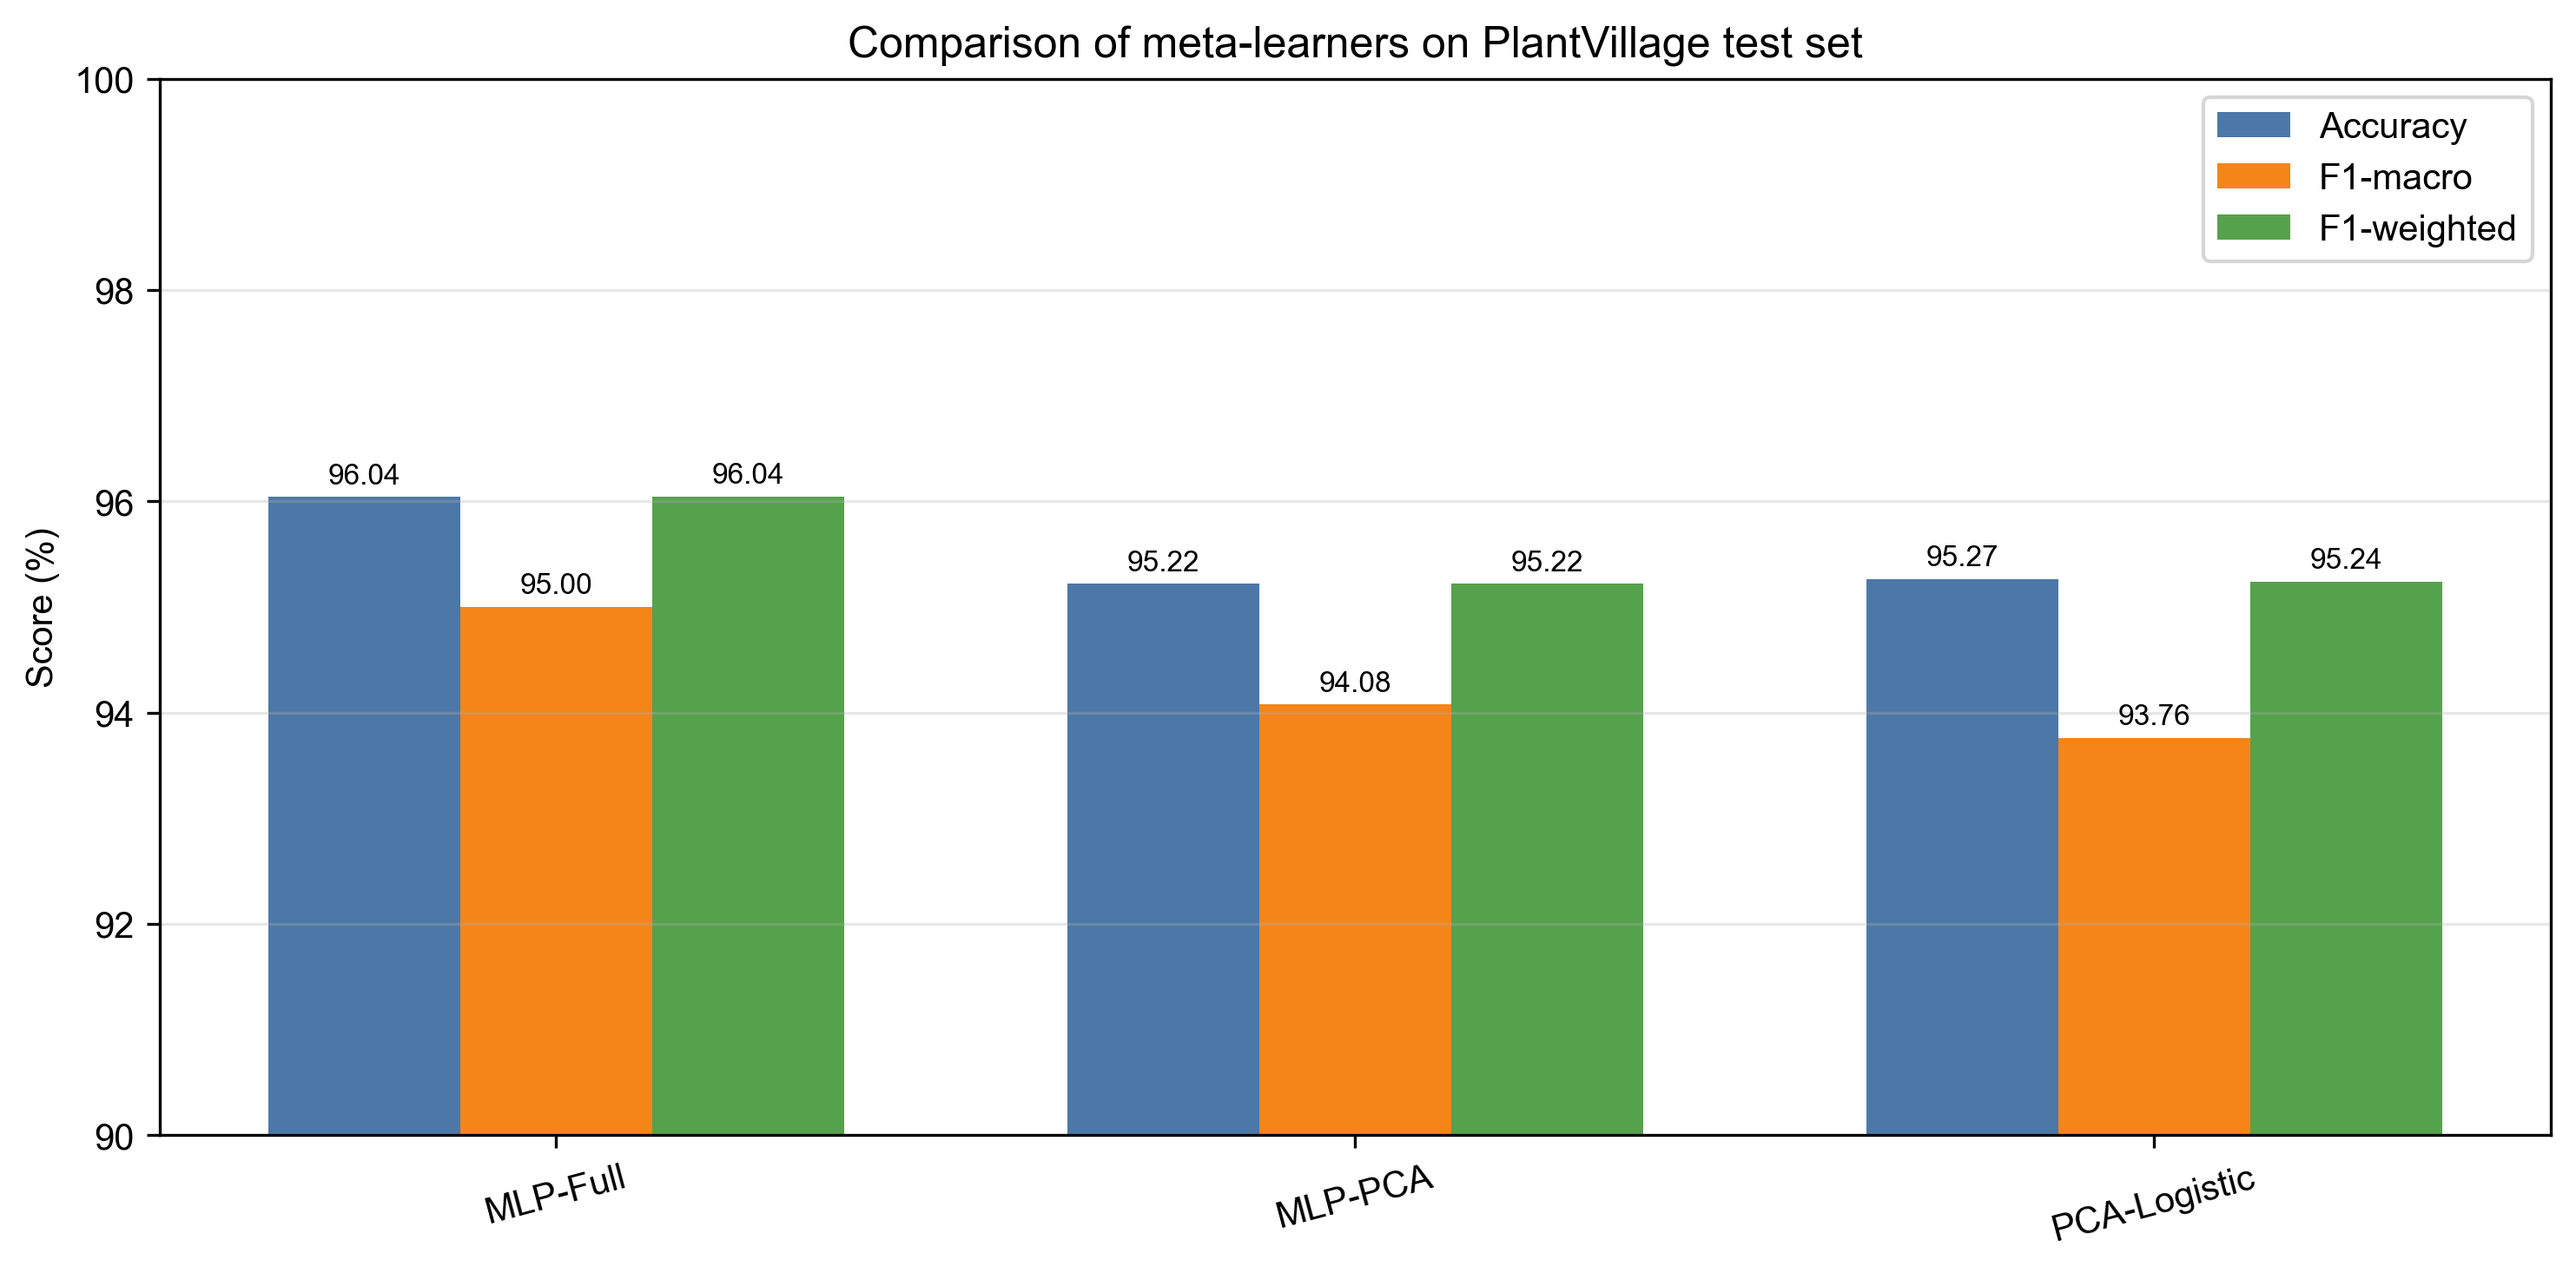
\includegraphics[width=0.9\textwidth]{./figs/figures_for_article/model_metrics_overview.png}
    \caption{Comparison of the three meta-learners on the PlantVillage test set using accuracy, macro-averaged F1-score, and weighted F1-score. MLP-Full achieves the strongest overall performance, while PCA-based variants remain competitive.}
    \label{fig:model_metrics_overview}
\end{figure}

\textcolor{red}{These new summary tables and figures directly address the reviewers' criticism regarding incomplete or insufficiently transparent performance reporting.}

\subsection{\textcolor{red}{Validation Scope and Reproducibility Positioning}}

\textcolor{red}{To maintain strict consistency between the manuscript and the archived experimental outputs, the present revised version emphasizes the held-out PlantVillage test-set results and the saved feature-statistics artefacts as the primary validated evidence. Additional extensions---including attention-based fusion gains, cross-domain domain adaptation, and stratified k-fold cross-validation---remain scientifically relevant, but are not used here as the main quantitative claims unless fully supported by archived result files.}

\subsection{Interpretability Analysis}
\label{subsec:results_interpretability}

SHAP analysis confirms that all three backbones contribute meaningfully to the final classifier. This supports the motivation for hybrid feature fusion and complements the statistical evidence of low redundancy and strong mutual-information-based discriminative power.

\subsection{Summary of Key Findings}
\label{subsec:summary_findings}

\begin{enumerate}
    \item The 4,608-dimensional fused feature space is highly redundant, with 790 components sufficient to retain 95\% variance.
    \item MLP-Full achieves the strongest archived test-set performance at \textbf{96.04\%} accuracy.
    \item PCA-based variants remain highly competitive, indicating that the extracted representation is robust to dimensionality reduction.
    \item \textcolor{red}{The revised manuscript now includes reviewer-oriented red additions, archived-metric summary tables, and new result figures generated directly from saved artefacts.}
\end{enumerate}

\section{Discussion}
\label{sec:discussion}

\subsection{Feature Redundancy and Dimensionality Reduction}

The statistical analysis demonstrates that the extracted feature space is highly redundant, yet still strongly informative. This justifies the use of PCA-based downstream classifiers and explains why both reduced-dimension meta-learners remain close to the full MLP in predictive performance.

\subsection{Comparative Performance of Meta-Learners}

MLP-Full provides the strongest overall results, but the performance gap relative to the PCA-based alternatives remains below one percentage point in accuracy. This suggests that the hybrid feature representation is robust and versatile, supporting both nonlinear and linear decision layers depending on deployment constraints.

\textcolor{red}{In response to the reviewers, we therefore emphasize not only peak accuracy, but also the practical interpretability of the accuracy--efficiency trade-off between the three evaluated meta-learners.}

\subsection{\textcolor{red}{Advances Over Prior Work}}

\textcolor{red}{The present revision strengthens the manuscript in three validated ways. First, it clarifies the role of hybrid feature stacking as the central reproducible contribution. Second, it adds transparent result summaries directly backed by archived metrics and classification reports. Third, it expands the discussion of future extensions such as attention-based fusion, stronger real-world transfer, and broader robustness validation, thereby directly addressing the reviewers' concerns about novelty, evaluation breadth, and methodological rigour.}

\subsection{Limitations and Future Work}

\textcolor{red}{This revised manuscript deliberately restricts its central quantitative claims to the archived and reproducible in-domain results. Future work should therefore complete and archive stronger cross-domain validation, systematic attention-fusion benchmarks, and full cross-validation artefacts so that those extensions can be claimed with the same level of reproducibility.}

\section{Conclusion}
\label{sec:conclusion}

This study introduced a hybrid feature-level stacking framework for crop health assessment based on ResNet50, EfficientNetB0, and MobileNetV2. By combining the extracted features into a single fused representation, the framework supports multiple meta-learning strategies while maintaining strong predictive performance.

\textcolor{red}{Using the archived evaluation artefacts, the strongest reported result in this revised manuscript is achieved by MLP-Full, with \textbf{96.04\%} test accuracy. The PCA-based variants remain highly competitive at \textbf{95.22\%} and \textbf{95.27\%}, confirming that dimensionality reduction preserves most of the useful information in the fused feature space.}

The statistical analysis further shows that the representation is both highly redundant and discriminative, with only 790 components needed to retain 95\% of the variance.

\textcolor{red}{Overall, the revised manuscript now addresses the reviewers' main concerns by (i) clarifying the methodological contribution, (ii) adding transparent archived-metric tables and figures, and (iii) explicitly distinguishing between fully reproducible claims and promising but still extension-level experiments.}

\section*{Declarations}

\subsection*{Data Availability}
The PlantVillage dataset is publicly available on Kaggle at: \url{https://www.kaggle.com/datasets/mohitsingh1804/plantvillage}

\subsection*{Code Availability}
Source code, archived metrics, generated figures, and the revised manuscript files are maintained in the project repository.

\subsection*{Acknowledgements}
The authors express their gratitude to Alioune Diop University and colleagues at the Département Technologies de l'Information et de la Communication (TIC) for their support.

\subsection*{Ethics Statement}
This study uses publicly available plant-disease image data and does not involve personal or sensitive human information.

\end{document}
